% Soubory musí být v kódování, které je nastaveno v příkazu \usepackage[...]{inputenc}

\documentclass[%        Základní nastavení
%  draft,    				  % Testovací překlad
  12pt,       				% Velikost základního písma je 12 bodů
  a4paper,    				% Formát papíru je A4
  %oneside,      			% Jednostranný tisk
    twoside,      			% Dvoustranný tisk (kapitoly a další důležité části tedy začínají na lichých stranách)
	unicode,						% Záložky a metainformace ve výsledném  PDF budou v kódování unicode
]{report}				    	% Dokument třídy 'zpráva', vhodná pro sazbu závěrečných prací s kapitolami

\usepackage[utf8]		  %	Kódování zdrojových souborů je UTF-8
	{inputenc}					% Balíček pro nastavení kódování zdrojových souborů

\usepackage{sectsty}
	%přetypuje nadpisy všech úrovní na bezpatkové, kromě \chapter, která je přenastavena zvlášť v thesis.sty
	\allsectionsfont{\sffamily}

\usepackage{graphicx} % Balíček 'graphicx' pro vkládání obrázků
											% Nutné pro vložení logotypů školy a fakulty

\usepackage[          % Balíček 'acronym' pro sazby zkratek a symbolů
	nohyperlinks				% Nebudou tvořeny hypertextové odkazy do seznamu zkratek
]{acronym}						
											% Nutné pro použití prostředí 'acronym' balíčku 'thesis'

\usepackage[
	breaklinks=true,		% Hypertextové odkazy mohou obsahovat zalomení řádku
	hypertexnames=false % Názvy hypertext. odkazů budou tvořeny nezávisle na názvech TeXu
]{hyperref}						% Balíček 'hyperref' pro sazbu hypertextových odkazů
											% Nutné pro použití příkazu 'pdfsettings' balíčku 'thesis'

\usepackage{pdfpages} % Balíček umožňující vkládat stránky z PDF souborů
                      % Nutné při vkládání titulních listů a zadání přímo
                      % ve formátu PDF z informačního systému

\usepackage{enumitem} % Balíček pro nastavení mezerování v odrážkách
  \setlist{topsep=0pt,partopsep=0pt,noitemsep} % konkrétní nastavení

\usepackage{cmap} 		% Balíček cmap zajišťuje, že PDF vytvořené `pdflatexem' je
											% plně "prohledávatelné" a "kopírovatelné"

%\usepackage{upgreek}	% Balíček pro sazbu stojatých řeckých písmem
											%% např. stojaté pí: \uppi
											%% např. stojaté mí: \upmu (použitelné třeba v mikrometrech)
											%% pozor, grafická nekompatibilita s fonty typu Computer Modern!
                      
%\usepackage{amsmath} %balíček pro sabu náročnější matematiky                 

\usepackage{dirtree}	% sazba adresářové struktury
                      % vhodné pro prezentaci obsahu elektronické přílohy (např. CD)

\usepackage[formats]{listings}	% Balíček pro sazbu zdrojových textů
\lstset{              % nastavení
%	Definice jazyka použitého ve výpisech
%    language=[LaTeX]{TeX},	% LaTeX
%	language={Matlab},		% Matlab
	language={C},           % jazyk C
    basicstyle=\ttfamily,	% definice základního stylu písma
    tabsize=2,			% definice velikosti tabulátoru
    inputencoding=utf8,         % pro soubory uložené v kódování UTF-8
		columns=fixed,  %fixed nebo flexible,
		fontadjust=true %licovani sloupcu
    extendedchars=true,
    literate=%  definice symbolů s diakritikou
    {á}{{\'a}}1
    {č}{{\v{c}}}1
    {ď}{{\v{d}}}1
    {é}{{\'e}}1
    {ě}{{\v{e}}}1
    {í}{{\'i}}1
    {ň}{{\v{n}}}1
    {ó}{{\'o}}1
    {ř}{{\v{r}}}1
    {š}{{\v{s}}}1
    {ť}{{\v{t}}}1
    {ú}{{\'u}}1
    {ů}{{\r{u}}}1
    {ý}{{\'y}}1
    {ž}{{\v{z}}}1
    {Á}{{\'A}}1
    {Č}{{\v{C}}}1
    {Ď}{{\v{D}}}1
    {É}{{\'E}}1
    {Ě}{{\v{E}}}1
    {Í}{{\'I}}1
    {Ň}{{\v{N}}}1
    {Ó}{{\'O}}1
    {Ř}{{\v{R}}}1
    {Š}{{\v{S}}}1
    {Ť}{{\v{T}}}1
    {Ú}{{\'U}}1
    {Ů}{{\r{U}}}1
    {Ý}{{\'Y}}1
    {Ž}{{\v{Z}}}1
}

%%%%%%%%%%%%%%%%%%%%%%%%%%%%%%%%%%%%%%%%%%%%%%%%%%%%%%%%%%%%%%%%%
%%%%%%      Definice informací o dokumentu             %%%%%%%%%%
%%%%%%%%%%%%%%%%%%%%%%%%%%%%%%%%%%%%%%%%%%%%%%%%%%%%%%%%%%%%%%%%%

% V tomto souboru se nastavují téměř veškeré informace, proměnné mezi studenty:
% jméno, název práce, pohlaví atd.
% Tento soubor je SDÍLENÝ mezi textem práce a prezentací k obhajobě -- netřeba něco nastavovat na dvou místech.

\usepackage[
%%% Z následujících voleb jazyka lze použít pouze jednu
  czech-english,		% originální jazyk je čeština, překlad je anglicky (výchozí)
  %english-czech,	% originální jazyk je angličtina, překlad je česky
  %slovak-english,	% originální jazyk je slovenština, překlad je anglicky
  %english-slovak,	% originální jazyk je angličtina, překlad je slovensky
%
%%% Z následujících voleb typu práce lze použít pouze jednu
  %semestral,		  % semestrální práce (výchozí)
  bachelor,			%	bakalářská práce
  %master,			  % diplomová práce
  %treatise,			% pojednání o disertační práci
  %doctoral,			% disertační práce
%
%%% Z následujících voleb zarovnání objektů lze použít pouze jednu
%  left,				  % rovnice a popisky plovoucích objektů budou zarovnány vlevo
	center,			    % rovnice a popisky plovoucích objektů budou zarovnány na střed (vychozi)
%
%%% Níže uvedený přepinač 'electronic' lze použít pro generování elektronické verze práce; pokud je aktivní, vnější a vnitřní okraj sazebního obrazce budou shodné pro liché i sudé stránky.
% Pozor, neplést si s volbou oneside/twoside!
% Pozor, pro tiskovou verzi nechejte vypnuté!
%    electronic			
]{thesis}   % Balíček pro sazbu studentských prací


%%% Jméno a příjmení autora ve tvaru
%  [tituly před jménem]{Křestní}{Příjmení}[tituly za jménem]
% Pokud osoba nemá titul před/za jménem, smažte celý řetězec '[...]'
\author{Luboš}{Kelnar}

%%% Identifikační číslo autora (VUT ID)
\butid{221 302}

%%% Pohlaví autora/autorky
% (nepoužije se ve variantě english-czech ani english-slovak)
% Číselná hodnota: 1...žena, 0...muž
\gender{0}

%%% Jméno a příjmení vedoucího/školitele včetně titulů
%  [tituly před jménem]{Křestní}{Příjmení}[tituly za jménem]
% Pokud osoba nemá titul před/za jménem, smažte celý řetězec '[...]'
\advisor[doc.\ Ing.]{Petr}{Fiedler}[Ph.D.]

%%% Jméno a příjmení oponenta včetně titulů
%  [tituly před jménem]{Křestní}{Příjmení}[tituly za jménem]
% Pokud osoba nemá titul před/za jménem, smažte celý řetězec '[...]'
% Nastavení oponenta se uplatní pouze v prezentaci k obhajobě;
% v případě, že nechcete, aby se na titulním snímku prezentace zobrazoval oponent, pouze příkaz zakomentujte;
% u obhajoby semestrální práce se oponent nezobrazuje (jelikož neexistuje)
% U dizertační práce jsou typicky dva až tři oponenti. Pokud je chcete mít na titulním slajdu, prosím ručně odkomentujte a upravte jejich jména v definici "VUT title page" v souboru thesis.sty.
%\opponent[doc.\ Mgr.]{Křestní}{Příjmení}[Ph.D.]

%%% Název práce
%  Parametr ve složených závorkách {} je název v originálním jazyce,
%  parametr v hranatých závorkách [] je překlad (podle toho jaký je originální jazyk).
%  V případě, že název Vaší práce je dlouhý a nevleze se celý do zápatí prezentace, použijte příkaz
%  \def\insertshorttitle{Zkác.\ náz.\ práce}
%  kde jako parametr vyplníte zkrácený název. Pokud nechcete zkracovat název, budete muset předefinovat,
%  jak se vytváří patička slidu. Viz odkaz: https://bit.ly/3EJTp5A
\title[Remote control and~visualization of a~demonstrative KNX panel]{Vzdálené řízení a~vizualizace demonstrativního panelu KNX}

%%% Označení oboru studia
%  Parametr ve složených závorkách {} je název oboru v originálním jazyce,
%  parametr v hranatých závorkách [] je překlad
\specialization[Automation and~Measurement]{Automatizační a~měřicí technika}

%%% Označení ústavu
%  Parametr ve složených závorkách {} je název ústavu v originálním jazyce,
%  parametr v hranatých závorkách [] je překlad
\department[Department of Control and Instrumentation]{Ústav automatizace a měřicí techniky}
%\department[Department of Biomedical Engineering]{Ústav biomedicínského inženýrství}
%\department[Department of Electrical Power Engineering]{Ústav elektroenergetiky}
%\department[Department of Electrical and Electronic Technology]{Ústav elektrotechnologie}
%\department[Department of Physics]{Ústav fyziky}
%\department[Department of Foreign Languages]{Ústav jazyků}
%\department[Department of Mathematics]{Ústav matematiky}
%\department[Department of Microelectronics]{Ústav mikroelektroniky}
%\department[Department of Radio Electronics]{Ústav radioelektroniky}
%\department[Department of Theoretical and Experimental Electrical Engineering]{Ústav teoretické a experimentální elektrotechniky}
%\department[Department of Telecommunications]{Ústav telekomunikací}
%\department[Department of Power Electrical and Electronic Engineering]{Ústav výkonové elektrotechniky a elektroniky}

%%% Označení fakulty
%  Parametr ve složených závorkách {} je název fakulty v originálním jazyce,
%  parametr v hranatých závorkách [] je překlad
%\faculty[Faculty of Architecture]{Fakulta architektury}
\faculty[Faculty of Electrical Engineering and~Communication]{Fakulta elektrotechniky a~komunikačních technologií}
%\faculty[Faculty of Chemistry]{Fakulta chemická}
%\faculty[Faculty of Information Technology]{Fakulta informačních technologií}
%\faculty[Faculty of Business and Management]{Fakulta podnikatelská}
%\faculty[Faculty of Civil Engineering]{Fakulta stavební}
%\faculty[Faculty of Mechanical Engineering]{Fakulta strojního inženýrství}
%\faculty[Faculty of Fine Arts]{Fakulta výtvarných umění}
%
%Nastavení logotypu (v hranatych zavorkach zkracene logo, ve slozenych plne):
\facultylogo[logo/FEKT_zkratka_barevne_PANTONE_CZ]{logo/UTKO_color_PANTONE_CZ}

%%% Rok odevzdání práce
\graduateyear{2025}
%%% Akademický rok odevzdání práce
\academicyear{2024/25}

%%% Datum obhajoby (uplatní se pouze v prezentaci k obhajobě)
\date{11.\,11.\,1980} 

%%% Místo obhajoby
% Na titulních stránkách bude automaticky vysázeno VELKÝMI písmeny (pokud tyto stránky sází šablona)
\city{Brno}

%%% Abstrakt
\abstract[%
The aim of this bachelor thesis is to implement remote control and visualization of a KNX demonstration panel using a TECO Programmable Logic Controller and modern display tools using Docker. The visualization is accessible through a web application optimized for mobile devices and tablets, with a clear menu divided into sections. The paper first introduces KNX technology and the possibilities of controlling the system, then describes the creation of control logic in ETS software and the possibilities of visualization using the automaton web server. Finally, alternative solutions using Raspberry Pi and Docker containers are discussed. The result is the design and implementation of a flexible system for remote control and monitoring of KNX installations.
]{%
Cílem této bakalářské práce je realizace vzdáleného řízení a vizualizace demonstračního panelu KNX pomocí programovatelného automatu společnosti TECO a moderních zobrazovacích nástrojů s využitím Dockeru. Vizualizace je dostupná prostřednictvím webové aplikace optimalizované pro mobilní zařízení a tablety, s přehledným menu rozděleným do sekcí. Práce nejprve seznamuje s technologií KNX a možnostmi řízení systému, dále popisuje tvorbu řídicí logiky v softwaru ETS a možnosti vizualizace pomocí webového serveru automatu. Závěrem jsou diskutována alternativní řešení s využitím Raspberry Pi a Docker kontejnerů. Výsledkem je návrh a implementace flexibilního systému pro vzdálené ovládání a monitorování KNX instalací.
}

%%% Klíčová slova
\keywrds[%
KNX, ETS, MQTT, Docker, visualization, intelligent wiring
]{%
KNX, ETS, MQTT, Docker, vizualizace, inteligentní elektroinstalace
}

%%% Poděkování
\acknowledgement{%
Rád bych poděkoval vedoucímu bakalářské práce
panu doc. Ing. Petru Fiedlerovi, Ph.D\ a konzultantu panu Ing. Branislavu Bátorovi Ph.D. za odborné vedení,
konzultace, trpělivost a~podnětné návrhy k~práci.
}%  % do tohoto souboru doplňte údaje o sobě, druhu práce, názvu...

%%%%%%%%%%%%%%%%%%%%%%%%%%%%%%%%%%%%%%%%%%%%%%%%%%%%%%%%%%%%%%%%%%%%%%%%

%%%%%%%%%%%%%%%%%%%%%%%%%%%%%%%%%%%%%%%%%%%%%%%%%%%%%%%%%%%%%%%%%%%%%%%%
%%%%%%     Nastavení polí ve Vlastnostech dokumentu PDF      %%%%%%%%%%%
%%%%%%%%%%%%%%%%%%%%%%%%%%%%%%%%%%%%%%%%%%%%%%%%%%%%%%%%%%%%%%%%%%%%%%%%
%% Při načteném balíčku 'hyperref' lze použít příkaz '\pdfsettings':
\pdfsettings
%  Nastavení polí je možné provést také ručně příkazem:
%\hypersetup{
%  pdftitle={Název studentské práce},    	% Pole 'Document Title'
%  pdfauthor={Autor studenstké práce},   	% Pole 'Author'
%  pdfsubject={Typ práce}, 						  	% Pole 'Subject'
%  pdfkeywords={Klíčová slova}           	% Pole 'Keywords'
%}
%%%%%%%%%%%%%%%%%%%%%%%%%%%%%%%%%%%%%%%%%%%%%%%%%%%%%%%%%%%%%%%%%%%%%%%

\pdfmapfile{=vafle.map}

%%%%%%%%%%%%%%%%%%%%%%%%%%%%%%%%%%%%%%%%%%%%%%%%%%%%%%%%%%%%%%%%%%%%%%%
%%%%%%%%%%%       Začátek dokumentu               %%%%%%%%%%%%%%%%%%%%%
%%%%%%%%%%%%%%%%%%%%%%%%%%%%%%%%%%%%%%%%%%%%%%%%%%%%%%%%%%%%%%%%%%%%%%%
\begin{document}
\pagestyle{empty} %vypnutí číslování stránek

%%% Vložení desek -- od září 2021 na žádost fakulty nepoužíváno
%\includepdf[pages=1]%  buďto generovaných informačním systémem
  %{pdf/student-desky}% název souboru nesmí obsahovat mezery!
%%% NEBO vytvoření desek z balíčku
%%\makecover
%%%
%\oddpage % při dvojstranném tisku přidá prázdnou stránku
%% kazdopádně ale:
%\setcounter{page}{1} %resetovaní čítače stránek -- desky do číslování nezahrnujeme

%% Vložení titulního listu
\includepdf[pages=1]%    buďto generovaného informačním systémem
  {pdf/student-titulka}% název souboru nesmí obsahovat mezery!
%% NEBO vytvoření titulní stránky z balíčku
%\maketitle
%%
\oddpage  % při dvojstranném tisku se přidá prázdná stránka
   
%% Vložení zadání
\includepdf[pages=1]%   buďto generovaného informačním systémem
  {pdf/student-zadani}% název souboru nesmí obsahovat mezery!
%% NEBO lze vytvořit prázdný list příkazem ze šablony
%\patternpage{}%
%	{\sffamily\Huge\centering ZDE VLOŽIT LIST ZADÁNÍ}%
%	{\sffamily\centering Z~důvodu správného číslování stránek}
%%
\oddpage% při dvojstranném tisku se přidá prázdná stránka

%% Vysázení stránky s abstraktem
\makeabstract

% Vysázení stránky s rozšířeným abstraktem
% (pokud píšete práci v češtině či slovenštině, vložení rozšířeného abstraktu zrušte;
%  pro semestrální projekt také není potřeba rozšířený abstrakt uvádět)
% Vysázení stránky s rozšířeným abstraktem
% (týká se pouze bc. a dp. prací psaných v angličtině, viz Směrnice rektora 72/2017)
\cleardoublepage
\noindent
{\large\sffamily\bfseries\MakeUppercase{Rozšířený abstrakt}}
\\
Výtah ze směrnice rektora 72/2017:\\
\emph{Bakalářská a diplomová práce předložená v angličtině musí obsahovat rozšířený abstrakt v češtině
nebo slovenštině (čl. 15). To se netýká studentů, kteří studují studijní program akreditovaný v
angličtině.}
(čl. 3, par. 7)\\
\emph{Nebude-li vnitřní normou stanoveno jinak, doporučuje se rozšířený abstrakt o rozsahu přibližně 3
normostrany, který bude obsahovat úvod, popis řešení a shrnutí a~zhodnocení výsledků.}
(čl. 15, par. 5)

%%% Vysázení citace práce
\makecitation

%%% Vysázení prohlášení o samostatnosti
\makedeclaration

%%% Vysázení poděkování
\makeacknowledgement

%%% Vysázení obsahu
\tableofcontents

%%% Vysázení seznamu obrázků
% (vynechejte, pokud máte dva nebo méně obrázků)
\listoffigures

%%% Vysázení seznamu tabulek
% (vynechejte, pokud máte dvě nebo méně tabulek)
\listoftables

%%% Vysázení seznamu výpisů kódu
% (vynechejte, pokud máte dva nebo méně výpisů)
\lstlistoflistings

\cleardoublepage\pagestyle{plain}   % zapnutí číslování stránek

%Pro vkládání kapitol i příloh používejte raději \include než \input
%%% Vložení souboru 'text/uvod.tex' s úvodem
\chapter*{Úvod}
\phantomsection
\addcontentsline{toc}{chapter}{Úvod}


Úvod studentské práce, např\,\dots

Nečíslovaná kapitola Úvod obsahuje \uv{seznámení} čtenáře s~problematikou práce.
Typicky se zde uvádí:
(a) do jaké tematické oblasti práce spadá, (b) co jsou hlavní cíle celé práce a (c) jakým způsobem jich bylo dosaženo.
Úvod zpravidla nepřesahuje jednu stranu.
Poslední odstavec Úvodu standardně představuje základní strukturu celého dokumentu.

Tato práce se věnuje oblasti \acs{DSP} (\acl{DSP}), zejména jevům, které nastanou při nedodržení Nyquistovy podmínky pro \ac{symfvz}.%
\footnote{Tato věta je pouze ukázkou použití příkazů pro sazbu zkratek.}

Šablona je nastavena na \emph{dvoustranný tisk}.
Nebuďte překvapeni, že ve vzniklém PDF jsou volné stránky.
Je to proto, aby důležité stránky jako např.\ začátky kapitol začínaly po vytisknutí a svázání vždy na pravé straně.
%
Pokud máte nějaký závažný důvod sázet (a~zejména tisknout) jednostranně, nezapomeňte si přepnout volbu \texttt{twoside} na \texttt{oneside}!

%%% Vložení souboru 'text/cile.tex' s úvodem
\chapter*{Cíle práce}
\phantomsection
\addcontentsline{toc}{chapter}{Cíle práce}

Cílem této bakalářské práce po domluvě s konzultantem je seznámení s technologií KNX, vytvoření programu pomocí softwaru ETS, naprogramování PLC a utvoření vizualizace skrze různé platformy.

%%% Vložení souboru 'text/reseni' s popisem řešení práce
% (rozdělte na více souborů či kapitol, pokud je vhodné)
\chapter{Teoretická část studentské práce}

Teoretické zázemí studentské práce vhodně rozdělené do částí.

(Struktura navržená v~této šabloně je nejhrubší možná, po konzultaci s~vedoucím je vhodné zvolit přiléhavější.)


%%% Vložení souboru 'text/vysledky' s popisem vysledků práce
% (rozdělte na více souborů či kapitol, pokud je vhodné)
\chapter{Výsledky studentské práce}

Praktická část a výsledky studentské práce vhodně rozdělené do částí.

\section{Programové řešení}
Lorem ipsum dolor sit amet, consectetuer adipiscing elit. Nulla pulvinar eleifend sem. Integer in sapien. Etiam sapien elit, consequat eget, tristique non, venenatis quis, ante. In laoreet, magna id viverra tincidunt, sem odio bibendum justo, vel imperdiet sapien wisi sed libero. Phasellus enim erat, vestibulum vel, aliquam a, posuere eu, velit. Aliquam erat volutpat. Nullam faucibus mi quis velit \cite{sr72/2017}.

\section{Výsledky měření}
Fusce tellus odio, dapibus id fermentum quis, suscipit id erat. Fusce tellus. Morbi scelerisque luctus velit. In laoreet, magna id viverra tincidunt, sem odio bibendum justo, vel imperdiet sapien wisi sed libero. Quisque porta. Fusce suscipit libero eget elit. Nulla non lectus sed nisl molestie malesuada. Phasellus faucibus molestie nisl. Integer vulputate sem a nibh rutrum consequat. Proin mattis lacinia justo. Phasellus et lorem id felis nonummy placerat. Etiam ligula pede, sagittis quis, interdum ultricies, scelerisque eu. Cras elementum. Aenean placerat. Donec ipsum massa, ullamcorper in, auctor et, scelerisque sed, est. Aliquam ante. Integer imperdiet lectus quis justo. Vivamus ac leo pretium faucibus. Nullam faucibus mi quis velit.

\subsection{Etiam quis quam}
Neque porro quisquam est, qui dolorem ipsum quia dolor sit amet, consectetur, adipisci velit, sed quia non numquam eius modi tempora incidunt ut labore et dolore magnam aliquam quaerat voluptatem. Aliquam erat volutpat. Lorem ipsum dolor sit amet, consectetuer adipiscing elit \cite{sr72/2017,pravidla}. Nunc auctor. Neque porro quisquam est, qui dolorem ipsum quia dolor sit amet, consectetur, adipisci velit, sed quia non numquam eius modi tempora incidunt ut labore et dolore magnam aliquam quaerat voluptatem. Maecenas lorem. Maecenas libero. In laoreet, magna id viverra tincidunt, sem odio bibendum justo, vel imperdiet sapien wisi sed libero. Nullam rhoncus aliquam metus.

\subsubsection{Integer rutrum orci vestibulum}
Integer rutrum, orci vestibulum ullamcorper ultricies, lacus quam ultricies odio, vitae placerat pede sem sit amet enim. Ut enim ad minim veniam, quis nostrud exercitation ullamco laboris nisi ut aliquip ex ea commodo consequat. Fusce tellus odio, dapibus id fermentum quis, suscipit id erat. Nullam eget nisl. Nunc auctor. Etiam dui sem, fermentum vitae, sagittis id, malesuada in, quam. Fusce dui leo, imperdiet in, aliquam sit amet, feugiat eu, orci. Curabitur vitae diam non enim vestibulum interdum. Aliquam erat volutpat. Pellentesque sapien. Phasellus enim erat, vestibulum vel, aliquam a, posuere eu, velit.

\subsubsection{Eger rutrum orci westibulum}
Fusce dui leo, imperdiet in, aliquam sit amet, feugiat eu, orci. Maecenas aliquet accumsan leo. Aliquam ornare wisi eu metus. Cum sociis natoque penatibus et magnis dis parturient montes, nascetur ridiculus mus. Aliquam erat volutpat. Donec iaculis gravida nulla. Sed elit dui, pellentesque a, faucibus vel, interdum nec, diam. Temporibus autem quibusdam et aut officiis debitis aut rerum necessitatibus saepe eveniet ut et voluptates repudiandae sint et molestiae non recusandae. Nulla non arcu lacinia neque faucibus fringilla. Phasellus enim erat, vestibulum vel, aliquam a, posuere eu, velit. Praesent vitae arcu tempor neque lacinia pretium
\cite{Walter1999,Svacina1999IEEE,RajmicSysel2002}.

Aliquam erat volutpat. Quisque porta. Integer imperdiet lectus quis justo. Nullam justo enim, consectetuer nec, ullamcorper ac, vestibulum in, elit. Nullam faucibus mi quis velit. Fusce tellus. Fusce consectetuer risus a nunc. Cras pede libero, dapibus nec, pretium sit amet, tempor quis. Morbi imperdiet, mauris ac auctor dictum, nisl ligula egestas nulla, et sollicitudin sem purus in lacus
\cite{CSN_ISO_690-2022,CSN_ISO_7144-1997,CSN_ISO_31-11}.
Mauris elementum mauris vitae tortor. Neque porro quisquam est, qui dolorem ipsum quia dolor sit amet, consectetur, adipisci velit, sed quia non numquam eius modi tempora incidunt ut labore et dolore magnam aliquam quaerat voluptatem. Quisque porta. Integer vulputate sem a nibh rutrum consequat. Nulla pulvinar eleifend sem. Praesent id justo in neque elementum ultrices \cite{Farkasova23:CSNISO6902022komentar}.

Fusce suscipit libero eget elit. Integer vulputate sem a nibh rutrum consequat. Aliquam erat volutpat. Etiam neque. Nulla turpis magna, cursus sit amet, suscipit a, interdum id, felis. Nullam rhoncus aliquam metus. Etiam dui sem, fermentum vitae, sagittis id, malesuada in, quam. Nunc auctor. Nunc dapibus tortor vel mi dapibus sollicitudin. Praesent in mauris eu tortor porttitor accumsan. Nulla non arcu lacinia neque faucibus fringilla. Nullam lectus justo, vulputate eget mollis sed, tempor sed magna. Maecenas lorem. Aenean placerat. Donec vitae arcu. Maecenas lorem. Donec iaculis gravida nulla. Nulla non lectus sed nisl molestie malesuada.

Duis pulvinar. Nulla est. Duis condimentum augue id magna semper rutrum. Integer pellentesque quam vel velit. Aliquam ante. Nulla quis diam. Proin mattis lacinia justo. Aenean fermentum risus id tortor. Nunc auctor. Nullam justo enim, consectetuer nec, ullamcorper ac, vestibulum in, elit. In dapibus augue non sapien. Etiam bibendum elit eget erat. In sem justo, commodo ut, suscipit at, pharetra vitae, orci. Maecenas libero.

Nulla non lectus sed nisl molestie malesuada. Donec vitae arcu. Aenean fermentum risus id tortor. Praesent in mauris eu tortor porttitor accumsan. Nulla pulvinar eleifend sem. Duis viverra diam non justo. Integer imperdiet lectus quis justo. Pellentesque habitant morbi tristique senectus et netus et malesuada fames ac turpis egestas. In rutrum. Excepteur sint occaecat cupidatat non proident, sunt in culpa qui officia deserunt mollit anim id est laborum. Nulla non lectus sed nisl molestie malesuada. Aliquam erat volutpat. Mauris tincidunt sem sed arcu. Duis bibendum, lectus ut viverra rhoncus, dolor nunc faucibus libero, eget facilisis enim ipsum id lacus. Fusce tellus odio, dapibus id fermentum quis, suscipit id erat. In enim a arcu imperdiet malesuada. Nulla non lectus sed nisl molestie malesuada. Proin mattis lacinia justo.

Aliquam in lorem sit amet leo accumsan lacinia. Cum sociis natoque penatibus et magnis dis parturient montes, nascetur ridiculus mus. Duis sapien nunc, commodo et, interdum suscipit, sollicitudin et, dolor. Suspendisse sagittis ultrices augue. Nullam lectus justo, vulputate eget mollis sed, tempor sed magna. In convallis. Praesent id justo in neque elementum ultrices. Neque porro quisquam est, qui dolorem ipsum quia dolor sit amet, consectetur, adipisci velit, sed quia non numquam eius modi tempora incidunt ut labore et dolore magnam aliquam quaerat voluptatem.

Pellentesque pretium lectus id turpis. Nemo enim ipsam voluptatem quia voluptas sit aspernatur aut odit aut fugit, sed quia consequuntur magni dolores eos qui ratione voluptatem sequi nesciunt. Curabitur ligula sapien, pulvinar a vestibulum quis, facilisis vel sapien. Praesent dapibus. Sed elit dui, pellentesque a, faucibus vel, interdum nec, diam. Duis viverra diam non justo. Duis ante orci, molestie vitae vehicula venenatis, tincidunt ac pede. Phasellus rhoncus. Maecenas fermentum, sem in pharetra pellentesque, velit turpis volutpat ante, in pharetra metus odio a lectus. Proin pede metus, vulputate nec, fermentum fringilla, vehicula vitae, justo. Fusce aliquam vestibulum ipsum. Nullam at arcu a est sollicitudin euismod.

%Aliquam ante. Phasellus faucibus molestie nisl. Etiam ligula pede, sagittis quis, interdum ultricies, scelerisque eu. Morbi leo mi, nonummy eget tristique non, rhoncus non leo. Cum sociis natoque penatibus et magnis dis parturient montes, nascetur ridiculus mus. Morbi scelerisque luctus velit. Curabitur bibendum justo non orci. Donec quis nibh at felis congue commodo. Nullam faucibus mi quis velit. Aenean id metus id velit ullamcorper pulvinar. Pellentesque sapien. Fusce nibh. Vestibulum fermentum tortor id mi. Nullam eget nisl. Praesent vitae arcu tempor neque lacinia pretium. Proin in tellus sit amet nibh dignissim sagittis. Donec quis nibh at felis congue commodo.
%
%Nam quis nulla. Proin in tellus sit amet nibh dignissim sagittis. Nullam dapibus fermentum ipsum. Curabitur ligula sapien, pulvinar a vestibulum quis, facilisis vel sapien. Nam libero tempore, cum soluta nobis est eligendi optio cumque nihil impedit quo minus id quod maxime placeat facere possimus, omnis voluptas assumenda est, omnis dolor repellendus. Vivamus ac leo pretium faucibus. Nunc tincidunt ante vitae massa. Maecenas sollicitudin. Ut tempus purus at lorem. Nullam lectus justo, vulputate eget mollis sed, tempor sed magna. Fusce consectetuer risus a nunc. Etiam quis quam.
%
%Donec quis nibh at felis congue commodo. Sed vel lectus. Donec odio tempus molestie, porttitor ut, iaculis quis, sem. Nullam feugiat, turpis at pulvinar vulputate, erat libero tristique tellus, nec bibendum odio risus sit amet ante. Sed elit dui, pellentesque a, faucibus vel, interdum nec, diam. Cras elementum. Sed vel lectus. Donec odio tempus molestie, porttitor ut, iaculis quis, sem. Etiam neque. Integer tempor. Vivamus porttitor turpis ac leo. Nulla non arcu lacinia neque faucibus fringilla.
%
%Etiam posuere lacus quis dolor. Nemo enim ipsam voluptatem quia voluptas sit aspernatur aut odit aut fugit, sed quia consequuntur magni dolores eos qui ratione voluptatem sequi nesciunt. Nullam faucibus mi quis velit. Cum sociis natoque penatibus et magnis dis parturient montes, nascetur ridiculus mus. Phasellus faucibus molestie nisl. Maecenas ipsum velit, consectetuer eu lobortis ut, dictum at dui. Maecenas aliquet accumsan leo. Pellentesque ipsum. Donec vitae arcu. Suspendisse nisl. Morbi imperdiet, mauris ac auctor dictum, nisl ligula egestas nulla, et sollicitudin sem purus in lacus. Pellentesque ipsum. Ut enim ad minima veniam, quis nostrum exercitationem ullam corporis suscipit laboriosam, nisi ut aliquid ex ea commodi consequatur? Nam libero tempore, cum soluta nobis est eligendi optio cumque nihil impedit quo minus id quod maxime placeat facere possimus, omnis voluptas assumenda est, omnis dolor repellendus.


%%% Vložení souboru 'text/zaver' se závěrem
\chapter*{Závěr}
\phantomsection
\addcontentsline{toc}{chapter}{Závěr}

V rámci této bakalářské práce byly splněny všechny stanovené cíle týkající se návrhu a realizace vzdáleného řízení a vizualizace demonstračního panelu KNX pro ovládání funkcí osvětlení, žaluzií, topení a klimatizace. Práce poskytuje ucelený pohled na problematiku sběrnicového systému KNX, jeho možnosti a praktické využití v oblasti domácí automatizace. 

V první části práce byla provedena důkladná analýza technologie KNX, včetně její historie, základních principů fungování, struktury komunikace, zabezpečení a topologie. Tato část poskytla nezbytný teoretický základ pro následnou praktickou realizaci. 

Druhá část práce se zaměřila na parametrizaci konkrétních přístrojů a tvorbu dynamických světelných scén. Byly popsány jednotlivé kroky od návrhu projektu až po jeho implementaci, včetně identifikace problémů. 

Třetí část práce se věnovala samotnému řízení a vizualizaci prostřednictvím PLC společnosti TECO. Popsány byly nejen technické aspekty programování a komunikace mezi PLC a KNX, ale také implementace MQTT protokolu a tvorba webové vizualizace. V této části práce vznikl problém těsně před jejím dokončením – došlo k poruše komunikační brány KNX IP BAOS 774. To mělo za následek nefunkčnost komunikace mezi PLC a KNX instalací. Situace je nyní řešena s technickou podporou a v nejhorším případě bude nutné vyměnit celou bránu.

V poslední části byly zhodnoceny možnosti využití open-source platforem pro vizualizaci a správu domácí automatizace. Byla provedena implementace na jednodeskovém počítači Raspberry Pi s využitím kontejnerizace Docker a nasazením několika open-source nástrojů, jako jsou Home Assistant, InfluxDB či Grafana. Tyto nástroje byly vybrány a nasazeny s ohledem na jejich aktuální popularitu, dostupnost a možnosti rozšíření.

Celkově lze konstatovat, že práce splnila vytyčené cíle a přinesla komplexní řešení vzdáleného řízení a vizualizace KNX panelu. Byly ověřeny možnosti integrace různých technologií a platforem, přičemž důraz byl kladen na praktičnost, flexibilitu a budoucí rozšiřitelnost řešení. Výsledky práce mohou sloužit jako inspirace či základ pro další rozvoj v oblasti chytré domácnosti a automatizace budov.


%%% Vložení souboru 'text/literatura' se seznamem zdrojů
% Pro sazbu seznamu literatury použijte jednu z následujících možností

%%%%%%%%%%%%%%%%%%%%%%%%%%%%%%%%%%%%%%%%%%%%%%%%%%%%%%%%%%%%%%%%%%%%%%%%%
%1) Seznam citací definovaný přímo pomocí prostředí literatura / thebibliography
\begin{thebibliography}{99}

\bibitem{Datapoint}
    	Asociace KNX \emph{Datapoint Type}\/ Online. 
    	Dostupné z:
    \url{https://support.knx.org/hc/en-us/articles/115001133744-Datapoint-Type}
    [cit.\,23.\,12.\,2021]. 
    
\bibitem{KNX history}
		Asociace KNX 
		\emph{A History of KNX}\/ Online.
		Dostupné z:
    \url{https://crelectrics.com.au/wp-content/uploads/2015/05/a_history_of_KNX.pdf}  
    [cit.\,1.\,10.\,2021]. 
    
\bibitem{KNX basics}
		Asociace KNX
		\emph{KNX Basics}\/ Online.
		Dostupné z:
    \url{https://www.knx.org/wAssets/docs/downloads/Marketing/Flyers/KNX-Basics/KNX-Basics_cz.pdf} 
		[cit.\,1.\,10.\,2021].
    
\bibitem{KNX principles}
    	Asociace KNX \emph{Principy systému KNX}\/ Online. 
    	Dostupné z:
    \url{https://knxcz.cz/images/clanky/KNX-System-Principles_cz.pdf} 
    	[cit.\,1.\,10.\,2021].
    
\bibitem{KNX Secure}
    	Asociace KNX \emph{KNX Secure Devices}\/ Online. 
    	Dostupné z:
    \url{https://support.knx.org/hc/en-us/articles/360000216419-KNX-Secure-Devices} 
    	[cit.\,23.\,12.\,2021].
    
\bibitem{Celkovy prehled}
    Asociace KNX \emph{ISO/IEC 14543-3. KNX Celkový přehled.}
    
\bibitem{Systemove Argumenty}
    Asociace KNX \emph{ISO/IEC 14543-3. KNX Systémové argumenty.}
    
\bibitem{Topologie}
    Asociace KNX \emph{ISO/IEC 14543-3. KNX TP Topologie.}
    
\bibitem{Mitrenga}
    MITRENGA, Michal.:
    \emph{Realizace demonstrativního panelu inteligentní elektroinstalace KNX. Brno, 2021.}\/ Online. 
    [cit. 26.\,12.\,2021].
    Dostupné z:
    \url{https://www.vutbr.cz/studenti/zav-prace/detail/134788}
    \emph{Diplomová práce. Vysoké učení technické v Brně, Fakulta elektrotechniky a komunikačních technologií, Ústav automatizace a měřicí techniky. Vedoucí práce Petr Fiedler.}
 
% \bibitem{Kalfus}
%    KALFUS, Petr..:
%    \emph{Návrh demonstračního panelu KNX. Brno, 2020.}\/ Online. 
%  [cit. 29.\,12.\,2021].
%   Dostupné z:
%    \url{https://www.vutbr.cz/studenti/zav-prace/detail/127255}   
%    \emph{Bakalářská práce. Vysoké učení technické v Brně, Fakulta elektrotechniky a komunikačních technologií, Ústav elektroenergetiky. Vedoucí práce Branislav Bátora.}

\bibitem{Asociace KNX}
		knx.org\/ Online.
		Dostupné z:
    \url{https://www.knx.org}
		[cit.\,1.\,10.\,2021]. 
    
\bibitem{ETS Kecy}
		knx.org \emph{ETS Professional}\/ Online.
		Dostupné z:
    \url{https://www.knx.org/knx-en/for-professionals/software/ets-professional/}
		[cit.\,2.\,1.\,2022]. 

\bibitem{KNXTunnel}
		Asociace KNX \emph{System Specifications KNXnet/IP - Tunelling}\/ Online.
		Dostupné z:
	\url{https://community-openhab-org.s3-eu-central-1.amazonaws.com/original/2X/8/8b3ec554f60872e37763d2005edc1c4c1fb16887.PDF}
		[cit.\,5.\,5.\,2025].

\bibitem{KNXRouting}
		Asociace KNX \emph{System Specifications - KNXnet/IP - Routing}\/ Online.
		Dostupné z:
	\url{https://community-openhab-org.s3-eu-central-1.amazonaws.com/original/2X/b/ba93de8a703a5ece40f0dfc1b596643cb28e8497.PDF}
		[cit.\,5.\,5.\,2025].

\bibitem{ABB}
		ABB - SBR/U6.0.1-84\/ Online. 
		Dostupné z:
    \url{https://new.abb.com/products/2CKA006330A0004/sbr-u6-0-1-84}
		[cit.\,28.\,12.\,2021].
    
\bibitem{ABB aktor1}
		ABB - SA/S8.10.2.1\/ Online.
		Dostupné z:
    \url{https://new.abb.com/products/2CDG110157R0011/sa-s8-10-2-1}
		[cit.\,28.\,12.\,2021]. 
    
\bibitem{ABB aktor2}
		ABB - JRA/S4.230.2.1\/ Online. 
		Dostupné z:
    \url{https://new.abb.com/products/2CDG110121R0011/jra-s4-230-2-1}
		[cit.\,28.\,12.\,2021].
    
\bibitem{Basalte}
		Basalte - Sentido aluminium - quad - Brushed black\/ Online.
		Dostupné z:
    \url{https://www.knxstore.cz/domu/1000403-basalte-sentido-aluminium-quad-brushed-black-5425025030224.html}
		[cit.\,28.\,12.\,2021]. 
    
 \bibitem{BEG}
		B.E.G - Indoor 140-L-KNX-DX\/ Online. 
		Dostupné z:
    \url{https://www.beg-luxomat.com/cz/produkty/luxomatnet/knx/knx-gen6-deluxe-pritomnostni-detektor/indoor-140-l-knx-dx/}
		[cit.\,28.\,12.\,2021].  
    
\bibitem{Berker}
		Berker - B.IQ push-button 3gang with thermostat Display, KNX\/ Online. 
		Dostupné z:
    \url{https://www.berker.com/en/e-catalogue/building-management-systems/knx-systems/berker-knx-system/b.iq-push-buttons-with-thermostat/75663593/355802.htm?lang=en}
		[cit.\,28.\,12.\,2021].
    
\bibitem{Ekinex}
		EKINEX - Pushbutton with thermostat\/ Online. 
		Dostupné z:
    \url{https://www.ekinex.com/en/15/pushbutton-with-thermostat.html}
		[cit.\,28.\,12.\,2021].
    
\bibitem{HDL}
        HDL - M/TBP6.1-A2-46 \textit{Ovládací prvek 6násobný iTouch, bílá}\/ Online. 
		Dostupné z:
    \url{https://b2b.hdl-automation.cz/cz/produkty/knx/ovladaci-prvky-hdl/ovladaci-prvky-itouch/hdl-m-tbp6-1-a2-46}
		[cit.\,28.\,12.\,2021].
    
\bibitem{HDL aktor1}
        HDL - M/R8.10.1 \textit{8CH 10A High Power Switch Actuator}\/ Online. 
		Dostupné z:
    \url{https://b2b.hdl-automation.cz/en/products/knx/switching-actuators/hdl-m-r8-10-1}
		[cit.\,28.\,12.\,2021].
    
\bibitem{HDL aktor2}
        HDL - M/DRGW4.1 \textit{Akční člen stmívací LED 4násobný, 7 A}\/ Online. 
		Dostupné z:
    \url{https://b2b.hdl-automation.cz/cz/produkty/knx/akcni-cleny-stmivaci/hdl-m-drgbw4-1}
		[cit.\,28.\,12.\,2021].
    
\bibitem{Siemens}
		SIEMENS - QMX3.P37 \textit{Prostorový KNX přístroj, displej pro regulaci HVAC, čidlo teploty, konfigurovatelná tlačítka pro osvětlení/žaluzie/scény}\/ Online. 
		Dostupné z:
    \url{https://hit.sbt.siemens.com/RWD/app.aspx?RC=CZ&lang=cs&MODULE=Catalog&ACTION=ShowProduct&KEY=S55624-H108}
		[cit.\,28.\,12.\,2021].
    
\bibitem{Siemens IP}
		SIEMENS - 5WG1 146-1AB03 \/ Online. 
		Dostupné z:
    \url{https://www.hqs.sbt.siemens.com/cps_product_data/data/search_find_en.htm?ssn=5WG11461AB03}
		[cit.\,28.\,12.\,2021].  
    
\bibitem{Simon}
		Simon \emph{Standard button box 4 functions white Simon 82 Sense}\/ Online. 
		Dostupné z:
    \url{https://www.simonelectric.com/intl/8000641-030-standard-button-box-4-functions-white-simon-82-sense.html}
		[cit.\,28.\,12.\,2021].

\bibitem{Weinzier}
		Weinzier - KNX IP BAOS 774\/ Online. 
		Dostupné z:
    \url{https://www.weinzierl.de/index.php/en/all-knx/knx-devices-en/knx-ip-baos-774-en}
		[cit.\,28.\,12.\,2021].
    
\bibitem{Weinzier ob}
		Weinzier - KNX IP BAOS 774 \emph{Rozhraní BAOS do 1000 bodů}\/ Online. 
		Dostupné z:
    \url{https://knx-trade.ru/weinzierl/597-5263.html}
		[cit.\,28.\,12.\,2021].

\bibitem{TECO}
		TECO - CP-2007\/ Online. 
		Dostupné z:
	\url{hhttps://wiki.tecomat.cz/clanek/cp-2007}
		[cit.\,23.\,4.\,2025].

\bibitem{Mosaic}
		TECO - Mosaic\/ Online. 
		Dostupné z:
	\url{https://www.tecomat.cz/ke-stazeni/software/mosaic/}
		[cit.\,23.\,4.\,2025].

\bibitem{IEC61131-3}
		TECO \emph{Programování PLC podle normy IEC 61 131-3 v prostředí Mosaic}\/ Online. 
		Dostupné z:
	\url{https://catalog.tecomat.cz/produkt/programovani-dle-normy-iec-61-131#download}
		[cit.\,23.\,4.\,2025].

\bibitem{KNXlib}
		TECO - Knihovna KnxLib\/ Online. 
		Dostupné z:
	\url{https://www.tecomat.cz/modules/DownloadManager/download.php?alias=txv00380_01}
		[cit.\,23.\,4.\,2025].

\bibitem{MQTT}
		MQTT \emph{The Standard for IoT Messaging}\/ Online. 
		Dostupné z:
	\url{https://mqtt.org}
		[cit.\,15.\,4.\,2025].

\bibitem{MQTTEsentials}
		MQTT Essentials \emph{The Ultimate Guide to MQTT for Beginners and Experts}\/ Online.
		Dostupné z:
		\url{https://www.hivemq.com/mqtt/}

\bibitem{JSON}
		JSON \emph{JavaScript Object Notation}\/ Online. 
		Dostupné z:
	\url{https://www.json.org/json-en.html}
		[cit.\,15.\,4.\,2025].

\bibitem{MQTTlib}
		TECO - Knihovna MQTTLib\/ Online. 
		Dostupné z:
	\url{https://support.tecomat.cz/storage/app/uploads/public/633/acd/862/633acd8625f3d859405244.pdf}
		[cit.\,23.\,4.\,2025].

\bibitem{WebMaker}
		TECO - WebMaker\/ Online. 
		Dostupné z:
	\url{https://www.tecomat.cz/modules/DownloadManager/download.php?alias=txv00328_01_mosaic_webmaker_cz}
		[cit.\,23.\,4.\,2025].

\bibitem{Flaticon}
		Flaticon \emph{The most wanted free SVG user interface icons}\/ Online. 
		Dostupné z:
	\url{https://www.flaticon.com/}
		[cit.\,5.\,5.\,2025].

\bibitem{Raspberry Pi 5}
		Raspberry Pi \emph{Raspberry Pi 5}\/ Online. 
		Dostupné z:
	\url{https://www.raspberrypi.com/products/raspberry-pi-5/}
		[cit.\,5.\,5.\,2025].

\bibitem{wear leveling}
		KIOXIA \emph{Managed Flash Background Operations Series - Part 3: Understanding Wear Leveling in NAND Flash Memory}\/ Online. 
		Dostupné z:
	\url{https://americas.kioxia.com/content/dam/kioxia/en-us/business/memory/mlc-nand/asset/KIOXIA_Managed_Flash_BOS_P3_Understanding_Wear_Leveling_Tech_Brief.pdf}
		[cit.\,5.\,5.\,2025].

\bibitem{Docker Compose}
		Docker Compose\/ Online. 
		Dostupné z:
	\url{https://docs.docker.com/compose/}
		[cit.\,5.\,5.\,2025].

\bibitem{DockerInstallationForDebian}
		Docker \emph{Docker Installation for Debian}\/ Online. 
		Dostupné z:
	\url{https://docs.docker.com/engine/install/debian/}
		[cit.\,5.\,5.\,2025].

\bibitem{ContainerAndVirtualization}
		Linux Containers \emph{Container and Virtualization tools}\/ Online.
		Dostupné z:
	\url{https://linuxcontainers.org}
		[cit.\,5.\,5.\,2025].

\bibitem{YAML}
		Yaml \emph{YAML Ain't Markup Language™}\/ Online. 
		Dostupné z:
	\url{hhttps://yaml.org/}
		[cit.\,5.\,5.\,2025].

\bibitem{ComposeYamlExample}
		Docker \emph{Compose file version 3 reference}\/ Online. 
		Dostupné z:
	\url{https://docs.docker.com/compose/compose-file/}
		[cit.\,5.\,5.\,2025].

\bibitem{ENV}
		Docker \emph{Environment variables}\/ Online. 
		Dostupné z:
	\url{https://docs.docker.com/engine/reference/run/#env}
		[cit.\,5.\,5.\,2025].

\bibitem{Portainer}
		Portainer\/ Online. 
		Dostupné z:
	\url{https://www.portainer.io/}
		[cit.\,5.\,5.\,2025].

\bibitem{Mosquitto}
		Eclipse Mosquitto\/ Online. 
		Dostupné z:
	\url{https://mosquitto.org/}
		[cit.\,15.\,5.\,2025].

\bibitem{Home Assistant}
		Home Assistant\/ Online. 
		Dostupné z:
	\url{https://www.home-assistant.io/}
		[cit.\,15.\,5.\,2025].

\bibitem{HACS}
		Home Assistant Community Store\/ Online. 
		Dostupné z:
	\url{https://hacs.xyz/}
		[cit.\,15.\,5.\,2025].

\bibitem{InfluxDB}
		InfluxDB\/ Online. 
		Dostupné z:
	\url{https://www.influxdata.com/}
		[cit.\,15.\,5.\,2025].

\bibitem{InfluxDBKeyConcepts}
		InfluxDB \emph{Key Concepts}\/ Online. 
		Dostupné z:
	\url{https://docs.influxdata.com/influxdb/v1/concepts/key_concepts/}
		[cit.\,15.\,5.\,2025].

\bibitem{Grafana}
		Grafana\/ Online. 
		Dostupné z:
	\url{https://grafana.com/}
		[cit.\,15.\,5.\,2025].

\bibitem{GrafanaVisualization}
		Grafana \emph{Visualizations}\/ Online. 
		Dostupné z:
	\url{https://grafana.com/docs/grafana/latest/panels-visualizations/visualizations/}
		[cit.\,15.\,5.\,2025].
\end{thebibliography} 
%%%%%%%%%%%%%%%%%%%%%%%%%%%%%%%%%%%%%%%%%%%%%%%%%%%%%%%%%%%%%%%%%%%%%%%%%
%%2) Seznam citací pomocí BibTeXu
%% Při použití je nutné v TeXnicCenter ve výstupním profilu aktivovat spouštění BibTeXu po překladu.
%% Definice stylu seznamu
%\bibliographystyle{unsrturl}
%% Pro českou sazbu lze použít styl czechiso.bst ze stránek
%% http://www.fit.vutbr.cz/~martinek/latex/czechiso.tar.gz
%%\bibliographystyle{czechiso}
%% Vložení souboru se seznamem citací
%\bibliography{text/literatura}
%
%% Následující příkaz je pouze pro ukázku sazby literatury při použití BibTeXu.
%% Způsobí citaci všech zdrojů v souboru literatura.bib, i když nejsou citovány v textu.
%\nocite{*}

%%% Vložení souboru 'text/zkratky' se seznam použitých symbolů, veličin a zkratek
\cleardoublepage
\chapter*{\listofabbrevname}
\phantomsection
\addcontentsline{toc}{chapter}{\listofabbrevname}

\begin{acronym}[KolikMista]

	\acro{zkTemp}		% název
		[Šířka levého sloupce Seznamu symbolů a zkratek]								% zkratka
		{je určena šířkou parametru prostředí \texttt{acronym} (viz řádek~1 výpisu zdrojáku na~str.\,\pageref{lst:zkratky})}
											% rozvinutí zkratky

	\acro{zkDummy}
		[KolikMista]
		{pouze ukázka vyhrazeného místa}

	\acro{DSP}		% název/zkratka
		{číslicové zpracování signálů -- Digital Signal Processing}
											% rozvinutí zkratky
	%%% bsymfvz
	\acro{symfvz}						% název
		[\ensuremath{f_\textind{vz}}] % symbol
		{vzorkovací kmitočet}					% popis
	%%% esymfvz

\end{acronym}


%%% Začátek příloh
\appendix

%%% Vysázení seznamu příloh
% (vynechejte, pokud máte dvě nebo méně příloh)
\listofappendices

%%% Vložení souboru 'text/prilohy' s přílohami
% Obvykle je přítomen alespoň popis co najdeme na přiloženém médiu
\chapter{Skupinové adresy}
\label{apend:skupinove_adresy}
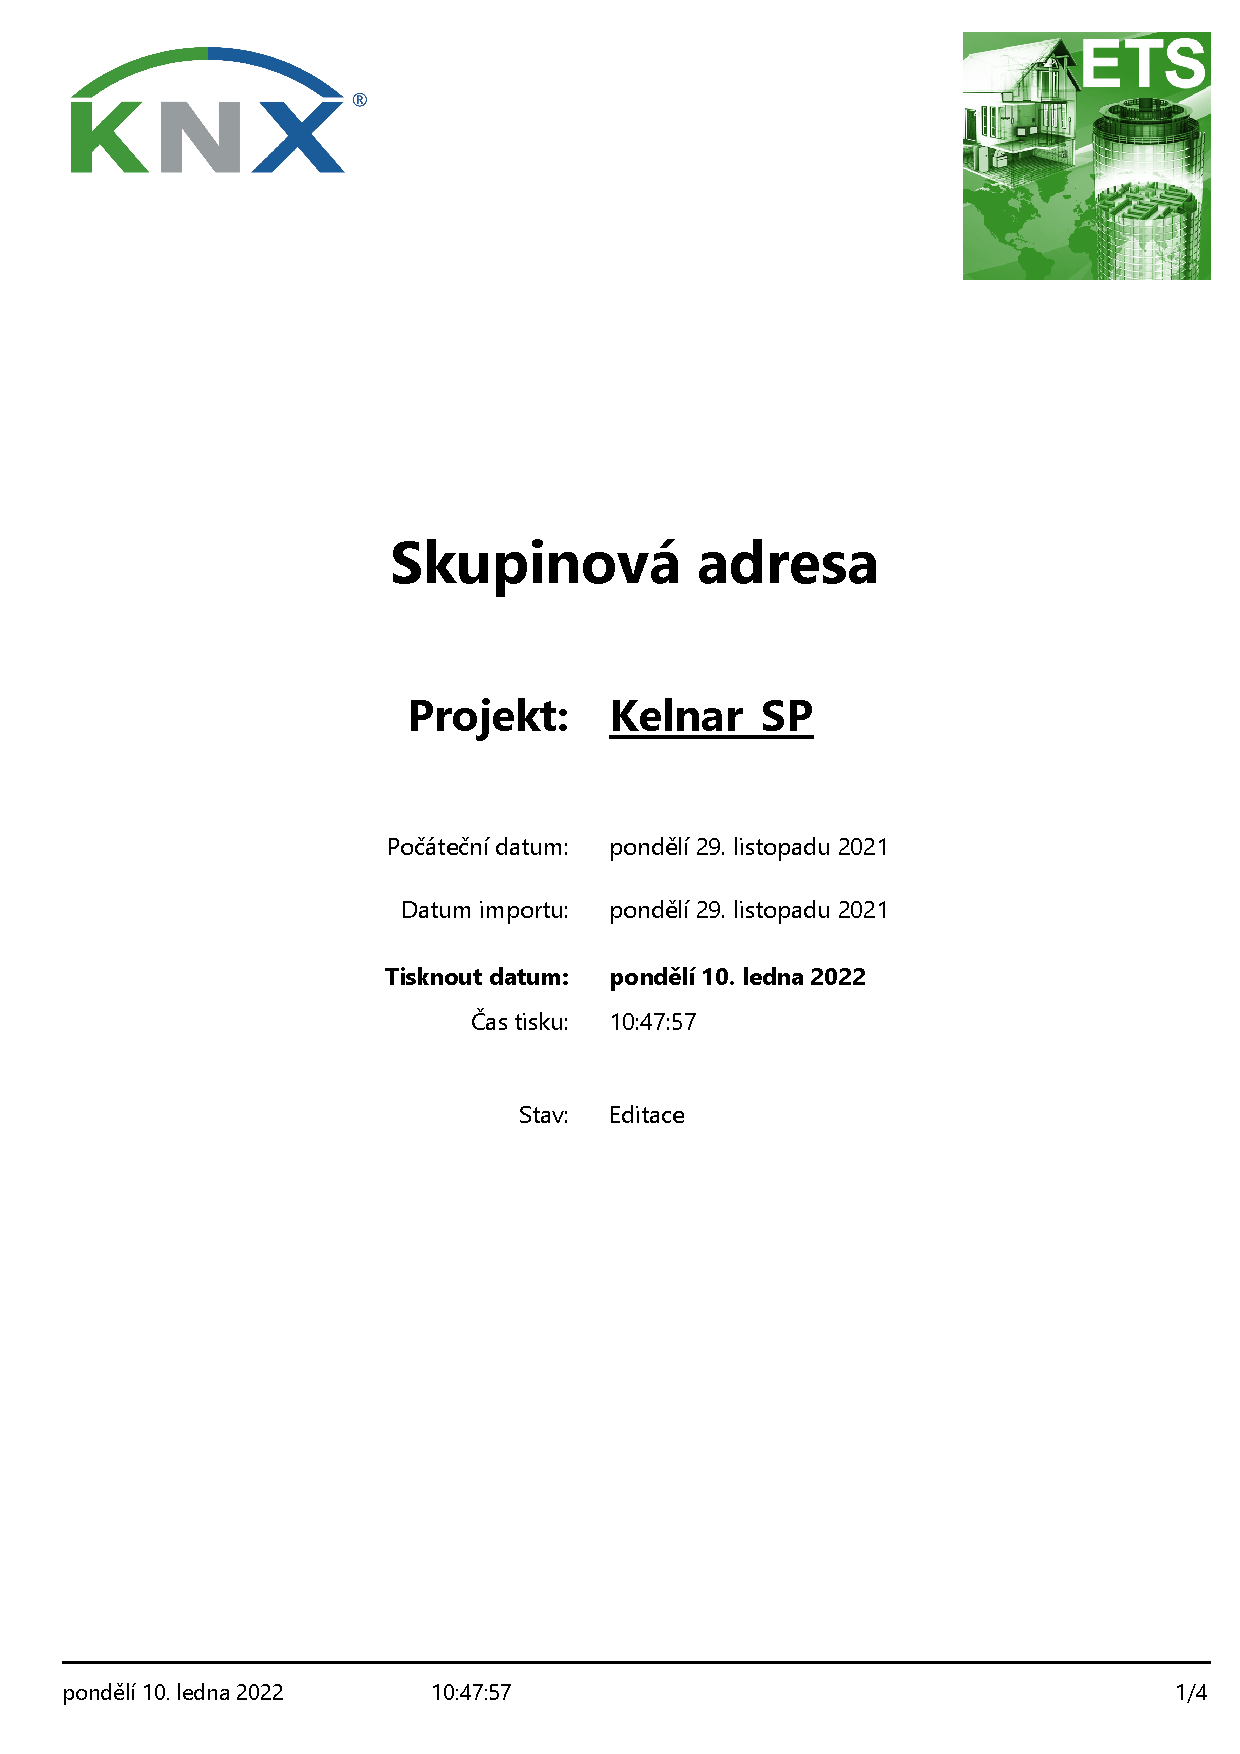
\includepdf[pages = 1]{pdf/GroupAddressesReport}
\includepdf[pages = 2]{pdf/GroupAddressesReport}
\includepdf[pages = 3]{pdf/GroupAddressesReport}
\includepdf[pages = 4]{pdf/GroupAddressesReport}
\chapter{Definice funkčního bloku fbRoomTempMod}
\label{apend:fbRoomTempMod}
\begin{lstlisting}[language=ST, breaklines=true, numbers=left, numberstyle=\small, numbersep=10pt, frame=single, basicstyle=\ttfamily\small, caption={Definice funkčního bloku fbRoomTempMod}, label={lst:fbRoomTempMod}]
(*
FUNCTION_BLOCK fbRoomTempMod
(*Simulace změny teploty v pokojích*)
  VAR_INPUT
    Heat_1       : BOOl; // Topení vstup 1 [-]
    Heat_1_WATTS : REAL; // Topení výkon 1 [W] => [J/s]
    Heat_2       : BOOL; // Topení vstup 2 [-]
    Heat_2_WATTS : REAL; // Topení výkon 2 [W] => [J/s]
    Cold_1       : BOOl; // Klimatizace vstup 1 [-]
    Cold_1_WATTS : REAL; // Klimatizace výkon 1 [W] => [J/s]
    Cold_2       : BOOL; // Klimatizace vstup 2 [-]
    Cold_2_WATTS : REAL; // Klimatizace výkon 2 [W] => [J/s]
    lenght       : REAL; // délka [m]
    width        : REAL; // šířka [m]
    height       : REAL; // výška [m]
    wall_temp1   : REAL; // Teplota za sousední zdí [deg C]
    wall_temp2   : REAL; // Teplota za sousední zdí [deg C]
    wall_temp3   : REAL; // Teplota za sousední zdí [deg C]
    wall_temp4   : REAL; // Teplota za sousední zdí [deg C]
    floor_temp   : REAL; // Teplota v místnosti pod [deg C]
    ceiling_temp : REAL; // Teplota v místnosti nad [deg C]
    wall_thic1   : REAL; // Šířka zdi1 [m]
    wall_thic2   : REAL; // Šířka zdi2 [m]
    wall_thic3   : REAL; // Šířka zdi3 [m]
    wall_thic4   : REAL; // Šířka zdi4 [m]
    floor_thic   : REAL; // Šířka podlahy [m]
    ceiling_thic : REAL; // Šířka stropu [m]
    TaskTime     : REAL; // Rychlost tasku [ms]
  END_VAR
  VAR_OUTPUT
    Temperature  : REAL := 20.0; // Teplota na výstupu [deg C]
  END_VAR
  VAR_IN_OUT
  END_VAR
  VAR
    INIT         : BOOL := FALSE; //INIT bloku
    TimeStep     : REAL := 0.0; // Hodnota kroku v ms
    VAir         : REAL := 0.0; // Obsah vzduchu v pokoji [m^3]
    MAir         : REAL := 0.0;  // Váha vzduchu [Kg]
    QAir         : REAL := 0.0; // Energie potřebná ke změně o 1deg C [J]
    RoomTemp     : REAL := 20.0; // Pokojová teplota [deg C]
    DeltaTemp    : REAL := 0.0; // Přírůstek teploty za jeden cyklus [deg C]
    KHeatRise    : REAL := 2.4; // Korekční člen pro rychlosti náběhu topení 1 [-]
    KColdRise    : REAL := 45.0; // Korekční člen pro rychlosti náběhu klimatizace 1 [-]
    KHeatFall1   : REAL := 0.0; // Korekční člen pro rychlost poklesu topení 1 [-]
    KColdFall1   : REAL := 0.0; // Korekční člen pro rychlost poklesu klimatizace 1 [-]
    KHeatFall2   : REAL := 0.0; // Korekční člen pro rychlost poklesu topení 2 [-]
    KColdFall2   : REAL := 0.0; // Korekční člen pro rychlost poklesu klimatizace 2 [-]
    Epsilon      : REAL := 1.0; // Hodnota pod kterou musí být výkon do stanoveného času [-]
    AlphaHeat    : REAL := 0.0; // Výsledek logaritmu pro topení [-]
    AlphaCold    : REAL := 0.0; // Výsledek logaritmu pro klimatizace [-]
    FiTotal      : REAL := 0.0; // Celkový tepelný tok [J/s]
    FiHeat       : REAL := 0.0; // Celkový tepelný tok topení [J/s]
    FiHeatTmp1   : REAL := 0.0; // Tepelný tok topení 1 teď [J/s]
    FiHeatTmp2   : REAL := 0.0; // Tepelný tok topení 2 teď [J/s]
    FiCold       : REAL := 0.0; // Celkový tepelný tok klimatizace [J/s]
    FiColdTmp1   : REAL := 0.0; // Tepelný tok klimatizace 1 teď [J/s]
    FiColdTmp2   : REAL := 0.0; // Tepelný tok klimatizace 2 teď [J/s]
    AreaWall1    : REAL := 0.0; // Plocha zdi 1 [m^2]
    AreaWall2    : REAL := 0.0; // Plocha zdi 2 [m^2]
    AreaWall3    : REAL := 0.0; // Plocha zdi 3 [m^2]
    AreaWall4    : REAL := 0.0; // Plocha zdi 4 [m^2]
    AreaFloor    : REAL := 0.0; // Plocha podlahy [m^2]
    AreaCeiling  : REAL := 0.0; // Plocha stropu [m^2]
  END_VAR
  VAR_TEMP
    DeltaTempWall_1     : REAL := 0; // Rozdíl teplot mezi pokoji 1 [deg C]
    DeltaTempWall_2     : REAL := 0; // Rozdíl teplot mezi pokoji 2 [deg C]
    DeltaTempWall_3     : REAL := 0; // Rozdíl teplot mezi pokoji 3 [deg C]
    DeltaTempWall_4     : REAL := 0; // Rozdíl teplot mezi pokoji 4 [deg C]
    DeltaTempFloor      : REAL := 0; // Rozdíl teplot mezi pokojem a podlahou [deg C]
    DeltaTempCeiling    : REAL := 0; // Rozdíl teplot mezi pokojem a stropem [deg C]
    FiWall_1     : REAL := 0.0; // Tepelný tok mezi pokoji 1 [J/s]
    FiWall_2     : REAL := 0.0; // Tepelný tok mezi pokoji 2 [J/s]
    FiWall_3     : REAL := 0.0; // Tepelný tok mezi pokoji 3 [J/s]
    FiWall_4     : REAL := 0.0; // Tepelný tok mezi pokoji 4 [J/s]
    FiFloor      : REAL := 0.0; // Tepelný tok mezi pokojem a podlahou [J/s]
    FiCeiling    : REAL := 0.0; // Tepelný tok mezi pokojem a stropem [J/s]
  END_VAR
  VAR CONSTANT
    RoAir        : REAL := 1.204; // Hustota vzduchu [Kg/m^3]
    CpAir        : REAL := 1005.0; // Tepelná kapacita vzduchu [J/(kg*K)]
    LambdaBrick  : REAL := 0.4; // Tepelná vodivost cihly [W/(m*K)]
    MaxTemp      : REAL := 24.0; // Maximální teplota [deg C]
    MinTemp      : REAL := 16.0; // Minimální teplota [deg C]
    TimeRise     : REAL := 15.0; // Čas náběhu výkonu [s]
    TimeFallHeat : REAL := 15.0; // Čas klesání výkonu topení [s]
    TimeFallCold : REAL := 10.0; // Čas klesání výkonu klimatizace [s]
    TargTimeHeat : REAL := 5.06; // Čas na dosažení 80% topení [s]
    TargTimeCold : REAL := 3.29; // Čas na dosažení 80% klimatizace [s]
  END_VAR
IF NOT(INIT) THEN
   TimeStep := TaskTime / 1000.0; // ms => s
END_IF;
(* Výpočet objemu, hmotnosti, energie *)
IF NOT(INIT) THEN
  VAir := lenght * width * height;
  MAir := RoAir * VAir;
  QAir := MAir * CpAir;
END_IF;

(* Výpočet ploch *)
IF NOT(INIT) THEN
  AreaWall1 := height * width;
  AreaWall2 := height * width;
  AreaWall3 := height * lenght;
  AreaWall4 := height * lenght;
  AreaFloor := lenght * width;
  AreaCeiling := lenght * width;
END_IF;

(* Výpočet deltaT *)
DeltaTempWall_1 := wall_temp1 - RoomTemp;
DeltaTempWall_2 := wall_temp2 - RoomTemp;
DeltaTempWall_3 := wall_temp3 - RoomTemp;
DeltaTempWall_4 := wall_temp4 - RoomTemp;
DeltaTempFloor := floor_temp - RoomTemp;
DeltaTempCeiling := ceiling_temp - RoomTemp;

(* Výpočet tepelných toků přes stěny *)
FiWall_1 := (LambdaBrick * AreaWall1 * DeltaTempWall_1) / wall_thic1;
FiWall_2 := (LambdaBrick * AreaWall2 * DeltaTempWall_2) / wall_thic2;
FiWall_3 := (LambdaBrick * AreaWall3 * DeltaTempWall_3) / wall_thic3;
FiWall_4 := (LambdaBrick * AreaWall4 * DeltaTempWall_4) / wall_thic4;
FiFloor := (LambdaBrick * AreaFloor * DeltaTempFloor) / floor_thic;
FiCeiling := (LambdaBrick * AreaCeiling * DeltaTempCeiling) / ceiling_thic;

(* Výpočet korekčních členu *)
IF NOT(INIT) THEN
  KHeatRise := (TimeRise / TargTimeHeat) - 1.0;
  KColdRise := (TimeRise / TargTimeCold) - 1.0;

  KHeatFall1 := (LN(Heat_1_WATTS/Epsilon))/TimeFallHeat;
  KHeatFall2 := (LN(Heat_2_WATTS/Epsilon))/TimeFallHeat;
  KColdFall1 := (LN(Cold_1_WATTS/Epsilon))/TimeFallCold;
  KColdFall2 := (LN(Cold_2_WATTS/Epsilon))/TimeFallCold;
END_IF;

(* Tepelný výkon topení a klimatizace *)
(* Výpočet alfy *)
IF NOT(INIT) THEN
  AlphaHeat := LN(1 + KHeatRise * (TimeStep)) / LN(1 + KHeatRise * TimeRise);
  AlphaCold := LN(1 + KColdRise * (TimeStep)) / LN(1 + KColdRise * TimeRise);
END_IF;

(* Topení 1 *)
IF Heat_1 THEN
  FiHeatTmp1 := FiHeatTmp1 + AlphaHeat * (Heat_1_WATTS - FiHeatTmp1);
ELSE
  FiHeatTmp1 := FiHeatTmp1 * EXP(-KHeatFall1 * (TimeStep));
END_IF;

(* Topení 2 *)
IF Heat_2 THEN
  FiHeatTmp2 := FiHeatTmp2 + AlphaHeat * (Heat_2_WATTS - FiHeatTmp2);
ELSE
  FiHeatTmp2 := FiHeatTmp2 * EXP(-KHeatFall2 * (TimeStep));
END_IF;

(* Klimatizace 1 *)
IF Cold_1 THEN
  FiColdTmp1 := FiColdTmp1 + AlphaCold * (Cold_1_WATTS - FiColdTmp1);
ELSE
  FiColdTmp1 := FiColdTmp1 * EXP(-KColdFall1 * (TimeStep));
END_IF;

(* Klimatizace 2 *)
IF Cold_2 THEN
  FiColdTmp2 := FiColdTmp2 + AlphaCold * (Cold_2_WATTS - FiColdTmp2);
ELSE
  FiColdTmp2 := FiColdTmp2 * EXP(-KColdFall2 * (TimeStep));
END_IF;

(* Suma výkonů *)
FiHeat := FiHeatTmp1 + FiHeatTmp2;
FiCold := FiColdTmp1 + FiColdTmp2;

(* Celkový tepelný tok *)
FiTotal := FiHeat - FiCold + FiWall_1 + FiWall_2 + FiWall_3 + FiWall_4 + FiFloor + FiCeiling;

(* Výpočet přírůstku teploty za task *)
DeltaTemp := (FiTotal / QAir) * TimeStep;
RoomTemp := RoomTemp + DeltaTemp;

(* Výstup *)
Temperature := RoomTemp;

(* NOT INIT *)
INIT := TRUE;
END_FUNCTION_BLOCK
\end{lstlisting}
\newpage
\chapter{Popis funkčního bloku fbBath}
\label{apend:fbBath}
\begin{lstlisting}[language=ST, breaklines=true, numbers=left, numberstyle=\small, numbersep=10pt, frame=single, basicstyle=\ttfamily\small, caption={Definice funkčního bloku fbBath}, label={lst:fbBath}]
  FUNCTION_BLOCK fbBath
  VAR_INPUT
    SV6_ON       : BOOl; //Vizu světlo 6 on
    SV6_OFF      : BOOl; //Vizu světlo 6 off
    SV6_KNX_FB   : BOOl; //KNX světlo 6 feedback
  END_VAR
  VAR_OUTPUT
    SV6          : BOOL;   //Vizualizace světla 6
    SV6_CMD      : DT_CMD_BOOL;   //Příkaz světla 6
    TemperBath   : REAL;   //Vizualizace + komunikace
  END_VAR
  VAR_IN_OUT
  END_VAR
  VAR
    Time_s   : REAL := 0.0;
    fbSV6 : fbKNXVisuBool;
  END_VAR
  VAR_TEMP
  END_VAR
  VAR CONSTANT
    PI       : REAL := 3.14159265;
    Freq     : REAL := 0.005; // perioda cca 3 minuty 20 sekund
    TaskTime : REAL := 400.0; // 250 ms
  END_VAR
\end{lstlisting}
\begin{figure}[!ht]
  \begin{center}
  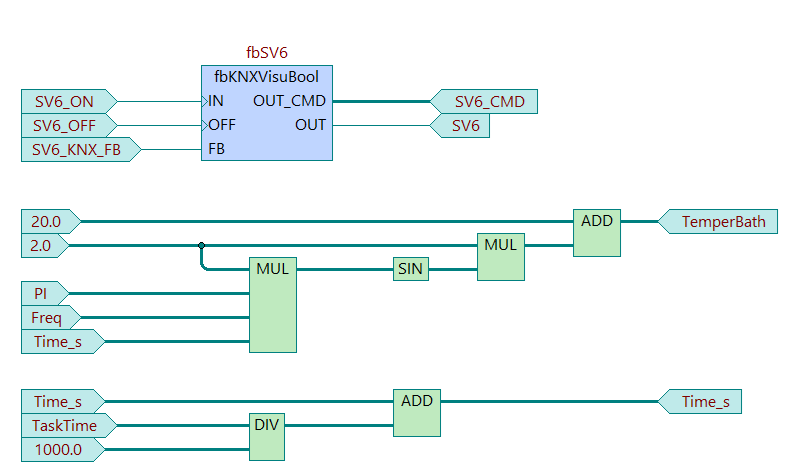
\includegraphics[scale=0.7]{obrazky/fbBath.png}
  \end{center}
  \caption[Logika funkčního bloku fbBath]{Logika funkčního bloku fbBath}
  \label{fig:fbBath}
\end{figure}
\pagebreak
\newpage
\chapter{Definice funkčního bloku fbKitch}
\label{apend:fbKitch}
\begin{lstlisting}[language=ST, breaklines=true, numbers=left, numberstyle=\small, numbersep=10pt, frame=single, basicstyle=\ttfamily\small, caption={Definice funkčního bloku fbKitch}, label={lst:fbKitch}]
  FUNCTION_BLOCK fbKitch
  VAR_INPUT
    SV1_ON         : BOOl; //Vizu světlo 1 on
    SV1_OFF        : BOOl; //Vizu světlo 1 off
    SV1_KNX_FB     : BOOl; //KNX světlo 1 feedback,
    SV2_ON         : BOOl; //Vizu světlo 2 on
    SV2_OFF        : BOOl; //Vizu světlo 2 off
    SV2_KNX_FB     : BOOl; //KNX světlo 2 feedback
    Heater3_ON     : BOOl; //Vizu topení 3 on
    Heater3_OFF    : BOOl; //Vizu topení 3 off
    Heater3_KNX_FB : BOOl; //KNX klimatizace 3 feedback
    Climat3_ON     : BOOl; //Vizu klimatizace 3 on
    Climat3_OFF    : BOOl; //Vizu klimatizace 3 off
    Climat3_KNX_FB : BOOl; //KNX topení 3 feedback
    wall_temp1     : REAL; // Teplota koupelna [deg C]
    wall_temp2     : REAL; // Teplota ven [deg C]
    wall_temp3     : REAL; // Teplota ven [deg C]
    wall_temp4     : REAL; // Teplota ven [deg C]
    ceiling_temp   : REAL; // Teplota obyvak [deg C]
  END_VAR
  VAR_OUTPUT
    SV1            : BOOL;   //Vizualizace světla 1
    SV2            : BOOL;   //Vizualizace světla 2
    Heater3        : BOOL;   //Vizualizace topení 3
    Climat3        : BOOL;   //Vizualizace klimatizace 3
    SV1_CMD        : DT_CMD_BOOL;   //Příkaz světla 1
    SV2_CMD        : DT_CMD_BOOL;   //Příkaz světla 2
    Heater3_CMD    : DT_CMD_BOOL;   //Příkaz topení 3
    Climat3_CMD    : DT_CMD_BOOL;   //Příkaz klimatizace 3
    TemperKitchen  : REAL;   //Vizualizace + komunikace
  END_VAR
  VAR_IN_OUT
  END_VAR
  VAR
    fbSV1 : fbKNXVisuBool;
    fbSV2 : fbKNXVisuBool;
    fbHeater3 : fbKNXVisuBool;
    fbKitchMod : fbRoomTempMod;
    fbClimat3 : fbKNXVisuBool;
  END_VAR
  VAR_TEMP
  END_VAR
\end{lstlisting}
\begin{figure}[!ht]
  \begin{center}
  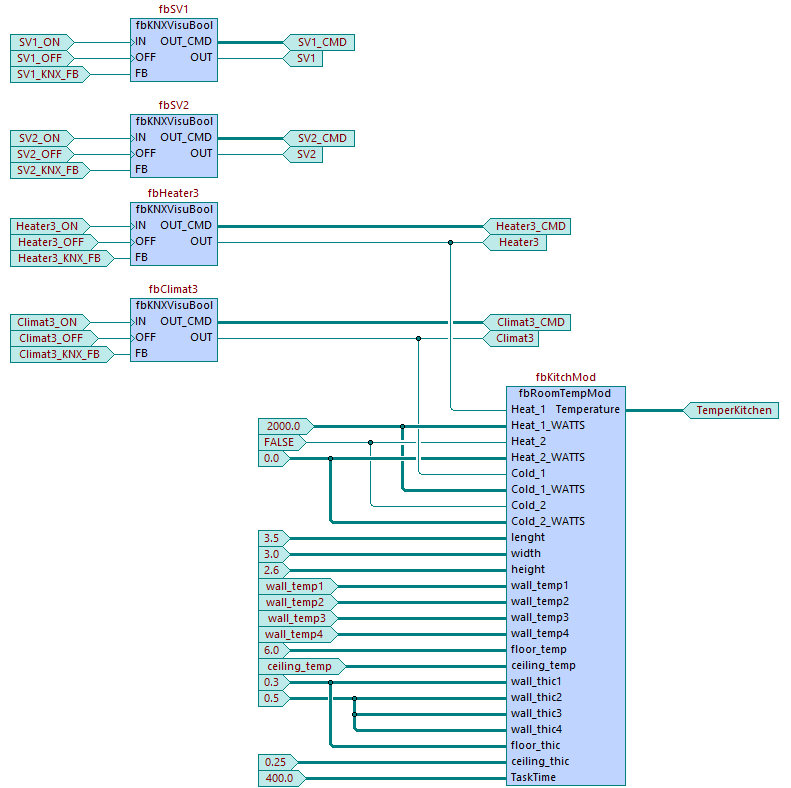
\includegraphics[scale=0.7]{obrazky/fbKitch.png}
  \end{center}
  \caption[Logika funkčního bloku fbKitch]{Logika funkčního bloku fbKitch}
  \label{fig:fbKitch}
\end{figure}
\pagebreak
\chapter{Definice funkčního bloku fbLivRoom}
\label{apend:fbLivRoom}
\begin{lstlisting}[language=ST, breaklines=true, numbers=left, numberstyle=\small, numbersep=10pt, frame=single, basicstyle=\ttfamily\small, caption={Definice funkčního bloku fbLivRoom}, label={lst:fbLivRoom}]
FUNCTION_BLOCK fbLivRoom
  VAR_INPUT
    SV3_ON          : BOOl; //Vizu světlo 3 on
    SV3_OFF         : BOOl; //Vizu světlo 3 off
    SV3_KNX_FB      : BOOl; //KNX světlo 3 feedback,
    SV4_ON          : BOOl; //Vizu světlo 4 on
    SV4_OFF         : BOOl; //Vizu světlo 4 off
    SV4_KNX_FB      : BOOl; //KNX světlo 4 feedback
    SV5_ON          : BOOl; //Vizu světlo 5 on
    SV5_OFF         : BOOl; //Vizu světlo 5 off
    SV5_KNX_FB      : BOOl; //KNX světlo 5 feedback
    Shut1_UP        : BOOl; //Vizu rolety 1 on
    Shut1_DW        : BOOl; //Vizu rolety 1 down
    Shut1_STEP_UP   : BOOl; //Vizu rolety 1 on krok
    Shut1_STEP_DW   : BOOl; //Vizu rolety 1 off krok
    Shut1_KNX_FB_UP : BOOl; //KNX rolety 1 feedback up
    Shut1_KNX_FB_DW : BOOl; //KNX rolety 1 feedback down
    Shut2_UP        : BOOl; //Vizu rolety 2 on
    Shut2_DW        : BOOl; //Vizu rolety 2 down
    Shut2_STEP_UP   : BOOl; //Vizu rolety 2 on krok
    Shut2_STEP_DW   : BOOl; //Vizu rolety 2 off krok
    Shut2_KNX_FB_UP : BOOl; //KNX rolety 2 feedback up
    Shut2_KNX_FB_DW : BOOl; //KNX rolety 2 feedback down
    Heater1_ON      : BOOl; //Vizu topení 1 on
    Heater1_OFF     : BOOl; //Vizu topení 1 off
    Heater1_KNX_FB  : BOOl; //KNX klimatizace 1 feedback
    Heater2_ON      : BOOl; //Vizu topení 2 on
    Heater2_OFF     : BOOl; //Vizu topení 2 off
    Heater2_KNX_FB  : BOOl; //KNX klimatizace 2 feedback
    Climat1_ON      : BOOl; //Vizu klimatizace 1 on
    Climat1_OFF     : BOOl; //Vizu klimatizace 1 off
    Climat1_KNX_FB  : BOOl; //KNX topení 1 feedback
    Climat2_ON      : BOOl; //Vizu klimatizace 2 on
    Climat2_OFF     : BOOl; //Vizu klimatizace 2 off
    Climat2_KNX_FB  : BOOl; //KNX topení 2 feedback
    wall_temp1      : REAL; // Teplota koupelna [deg C]
    wall_temp2      : REAL; // Teplota ven [deg C]
    wall_temp3      : REAL; // Teplota ven [deg C]
    wall_temp4      : REAL; // Teplota ven [deg C]
    floor_temp      : REAL; // Teplota v místnosti pod [deg C]
    ceiling_temp    : REAL; // Teplota obyvak [deg C]
  END_VAR
  VAR_OUTPUT
    SV3          : BOOL;   //Vizualizace světla 3
    SV4          : BOOL;   //Vizualizace světla 4
    SV5          : BOOL;   //Vizualizace světla 5
    SV3_CMD      : DT_CMD_BOOL;   //Příkaz světla 3
    SV4_CMD      : DT_CMD_BOOL;   //Příkaz světla 4
    SV5_CMD      : DT_CMD_BOOL;   //Příkaz světla 5
    Heater1        : BOOL;   //Vizualizace topení 1
    Heater2        : BOOL;   //Vizualizace topení 2
    Heater1_CMD    : DT_CMD_BOOL;   //Příkaz topení 1
    Heater2_CMD    : DT_CMD_BOOL;   //Příkaz topení 2
    Climat1        : BOOL;   //Vizualizace klimatizace 1
    Climat2        : BOOL;   //Vizualizace klimatizace 2
    Climat1_CMD    : DT_CMD_BOOL;   //Příkaz klimatizace 1
    Climat2_CMD    : DT_CMD_BOOL;   //Příkaz klimatizace 2
    Shut1_UP_OUT   : BOOL;   //Vizualizace žaluzie 1 UP
    Shut1_DOWN_OUT : BOOL;   //Vizualizace žaluzie 1 DOWN
    Shut1_CMD      : DT_CMD_BOOL;   //Příkaz žaluzie 1
    Shut1_STEP_CMD : DT_CMD_BOOL;   //Příkaz žaluzie 1 KROK
    Shut2_UP_OUT   : BOOL;   //Vizualizace žaluzie 2 UP
    Shut2_DOWN_OUT : BOOL;   //Vizualizace žaluzie 2 DOWN
    Shut2_CMD      : DT_CMD_BOOL;   //Příkaz žaluzie 2
    Shut2_STEP_CMD : DT_CMD_BOOL;   //Příkaz žaluzie 2 KROK
    TemperLivingR  : REAL;   //Vizualizace + komunikace
  END_VAR
  VAR_IN_OUT
  END_VAR
  VAR
    fbSV3 : fbKNXVisuBool;
    fbSV4 : fbKNXVisuBool;
    fbSV5 : fbKNXVisuBool;
    fbHeater1 : fbKNXVisuBool;
    fbClimat1 : fbKNXVisuBool;
    fbHeater2 : fbKNXVisuBool;
    fbClimat2 : fbKNXVisuBool;
    fbLivingRMod : fbRoomTempMod;
    fbShut1 : fbKNXShutters;
    fbShut2 : fbKNXShutters;
  END_VAR
  VAR_TEMP
  END_VAR
\end{lstlisting}
\begin{figure}[!ht]
  \begin{center}
  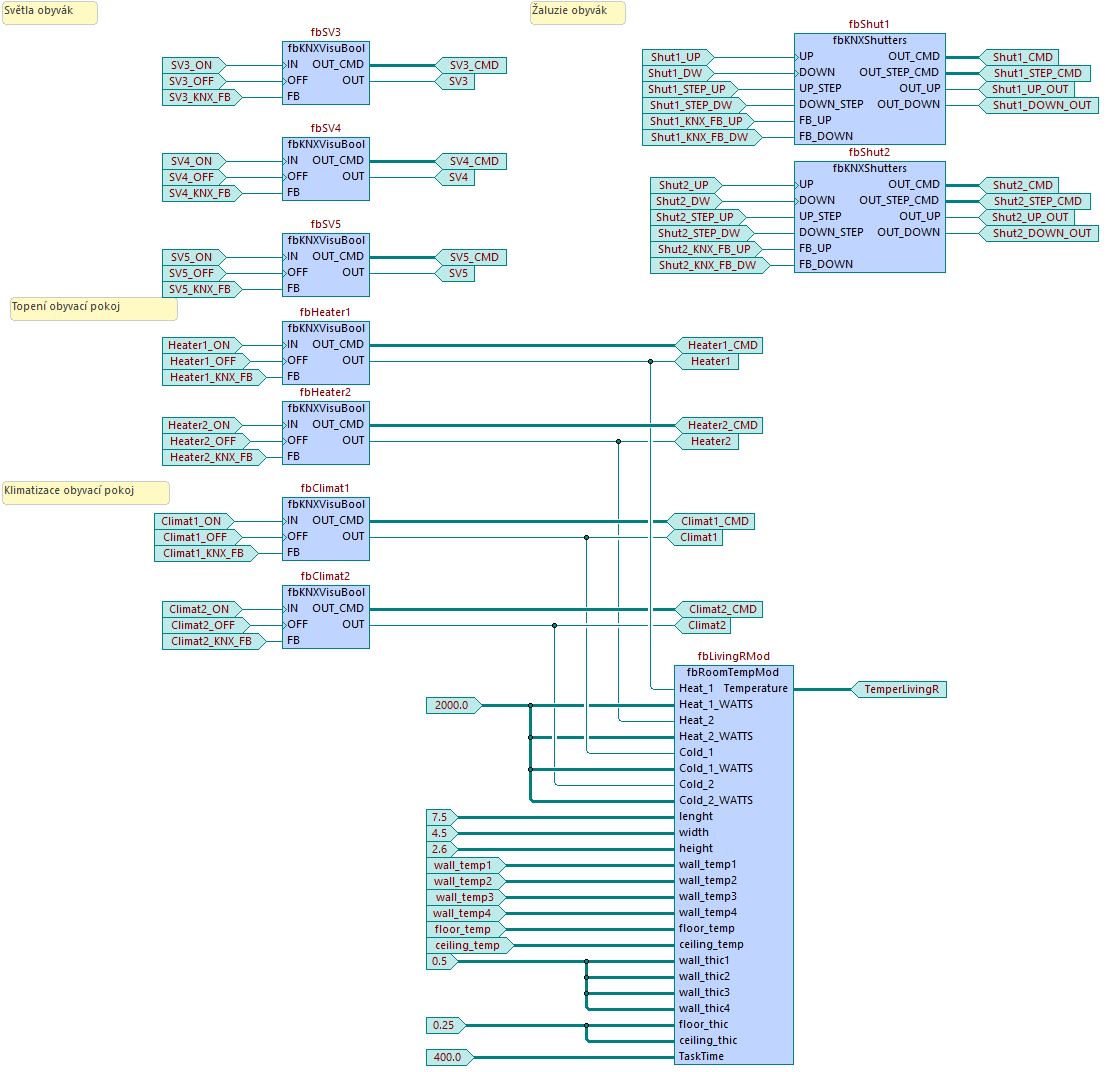
\includegraphics[scale=0.6]{obrazky/fbLivRoom.png}
  \end{center}
  \caption[Logika funkčního bloku fbLivRoom]{Logika funkčního bloku fbLivRoom}
  \label{fig:fbLivRoom}
\end{figure}
\pagebreak
\chapter{Definice funkčního bloku fbOutz}
\label{apend:fbOutz}
\begin{lstlisting}[language=ST, breaklines=true, numbers=left, numberstyle=\small, numbersep=10pt, frame=single, basicstyle=\ttfamily\small, caption={Definice funkčního bloku fbOutz}, label={lst:fbOutz}]
  FUNCTION_BLOCK fbOutz
  VAR_INPUT
    SV7_ON       : BOOl R_EDGE; //Vizu světlo 7 on
    SV7_OFF      : BOOl R_EDGE; //Vizu světlo 7 off
    SV7_KNX_FB   : BOOl; //KNX světlo 7 feedback
    KNX_OUT_TEMP : REAL; // KNX Teplota venku
  END_VAR
  VAR_OUTPUT
    SV7          : BOOL;   //Vizualizace světla 7
    SV7_CMD      : DT_CMD_BOOL;   //Příkaz světla 7
    TemperOut    : REAL;   //Vizualizace + komunikace
  END_VAR
  VAR_IN_OUT
  END_VAR
  VAR
    fbSV7 : fbKNXVisuBool;
  END_VAR
  VAR_TEMP
  END_VAR
\end{lstlisting}
\begin{figure}[!ht]
  \begin{center}
  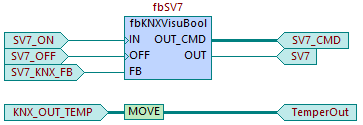
\includegraphics[scale=1.3]{obrazky/fbOutz.png}
  \end{center}
  \caption[Logika funkčního bloku fbOutz]{Logika funkčního bloku fbOutz}
  \label{fig:fbOutz}
\end{figure}
\pagebreak
\chapter{Program komunikace mezi PLC a KNX}
\label{apend:KNXComm}
\begin{lstlisting}[language=ST, breaklines=true, numbers=left, numberstyle=\small, numbersep=10pt, frame=single, basicstyle=\ttfamily\small, caption={Program komunikace mezi PLC a KNX}, label={lst:prgKNXComm}]
  PROGRAM prgKNXComm
  VAR_INPUT
  END_VAR
  VAR_OUTPUT
  END_VAR
  VAR
    init : BOOL;
    knx  : fbKnxIpBaosBin;
    
    SHUT1_FB_PULSE : TON;
    SHUT2_FB_PULSE : TON;

    datapoint1       : T_KNX_OBJECT_DPT1;     // SV1_FB
    datapoint2       : T_KNX_OBJECT_DPT1;     // SV2_FB
    datapoint3       : T_KNX_OBJECT_DPT1;     // SV3_FB
    datapoint4       : T_KNX_OBJECT_DPT1;     // SV4_FB
    datapoint5       : T_KNX_OBJECT_DPT1;     // SV5_FB
    datapoint6       : T_KNX_OBJECT_DPT1;     // SV6_FB
    datapoint7       : T_KNX_OBJECT_DPT1;     // SV7_FB

    datapoint8       : T_KNX_OBJECT_DPT1;     // HEAT1_FB
    datapoint9       : T_KNX_OBJECT_DPT1;     // HEAT2_FB
    datapoint10      : T_KNX_OBJECT_DPT1;     // HEAT3_FB

    datapoint11      : T_KNX_OBJECT_DPT1;     // COLD1_FB
    datapoint12      : T_KNX_OBJECT_DPT1;     // COLD2_FB
    datapoint13      : T_KNX_OBJECT_DPT1;     // COLD3_FB

    datapoint14      : T_KNX_OBJECT_DPT1;     // SHUT1_FB
    datapoint15      : T_KNX_OBJECT_DPT1;     // SHUT1_CMD
    datapoint16      : T_KNX_OBJECT_DPT1;     // SHUT2_FB
    datapoint17      : T_KNX_OBJECT_DPT1;     // SHUT2_CMD

    datapoint18      : T_KNX_OBJECT_DPT1;     // SV1_CMD
    datapoint19      : T_KNX_OBJECT_DPT1;     // SV2_CMD
    datapoint20      : T_KNX_OBJECT_DPT1;     // SV3_CMD
    datapoint21      : T_KNX_OBJECT_DPT1;     // SV4_CMD
    datapoint22      : T_KNX_OBJECT_DPT1;     // SV5_CMD
    datapoint23      : T_KNX_OBJECT_DPT1;     // SV6_CMD
    datapoint24      : T_KNX_OBJECT_DPT1;     // SV7_CMD

    datapoint25      : T_KNX_OBJECT_DPT1;     // HEAT1_CMD
    datapoint26      : T_KNX_OBJECT_DPT1;     // HEAT2_CMD
    datapoint27      : T_KNX_OBJECT_DPT1;     // HEAT3_CMD

    datapoint28      : T_KNX_OBJECT_DPT1;     // krok Žaluzií 1
    datapoint29      : T_KNX_OBJECT_DPT1;     // krok Žaluzií 2

    datapoint30      : T_KNX_OBJECT_DPT18;    // scéna
    datapoint31      : T_KNX_OBJECT_DPT9;     // teplota

    knxObjectList    : ARRAY[1..31] OF UDINT; // pole adres
  END_VAR
  VAR_TEMP
  END_VAR
  
// pole adres
IF NOT init THEN
  knxObjectList[1]  := PTR_TO_UDINT( ADR(datapoint1));   // SV1_FB
  knxObjectList[2]  := PTR_TO_UDINT( ADR(datapoint2));   // SV2_FB
  knxObjectList[3]  := PTR_TO_UDINT( ADR(datapoint3));   // SV3_FB
  knxObjectList[4]  := PTR_TO_UDINT( ADR(datapoint4));   // SV4_FB
  knxObjectList[5]  := PTR_TO_UDINT( ADR(datapoint5));   // SV5_FB
  knxObjectList[6]  := PTR_TO_UDINT( ADR(datapoint6));   // SV6_FB
  knxObjectList[7]  := PTR_TO_UDINT( ADR(datapoint7));   // SV7_FB

  knxObjectList[8]  := PTR_TO_UDINT( ADR(datapoint8));   // HEAT1_FB
  knxObjectList[9]  := PTR_TO_UDINT( ADR(datapoint9));   // HEAT2_FB
  knxObjectList[10] := PTR_TO_UDINT( ADR(datapoint10));  // HEAT3_FB

  knxObjectList[11] := PTR_TO_UDINT( ADR(datapoint11));  // COLD1_FB
  knxObjectList[12] := PTR_TO_UDINT( ADR(datapoint12));  // COLD2_FB
  knxObjectList[13] := PTR_TO_UDINT( ADR(datapoint13));  // COLD3_FB

  knxObjectList[14] := PTR_TO_UDINT( ADR(datapoint14));  // SHUT1_FB
  knxObjectList[15] := PTR_TO_UDINT( ADR(datapoint15));  // Zastarale
  knxObjectList[16] := PTR_TO_UDINT( ADR(datapoint16));  // SHUT2_FB
  knxObjectList[17] := PTR_TO_UDINT( ADR(datapoint17));  // Zastarale

  knxObjectList[18] := PTR_TO_UDINT( ADR(datapoint18));  // SV1_CMD
  knxObjectList[19] := PTR_TO_UDINT( ADR(datapoint19));  // SV2_CMD
  knxObjectList[20] := PTR_TO_UDINT( ADR(datapoint20));  // SV3_CMD
  knxObjectList[21] := PTR_TO_UDINT( ADR(datapoint21));  // SV4_CMD
  knxObjectList[22] := PTR_TO_UDINT( ADR(datapoint22));  // SV5_CMD
  knxObjectList[23] := PTR_TO_UDINT( ADR(datapoint23));  // SV6_CMD
  knxObjectList[24] := PTR_TO_UDINT( ADR(datapoint24));  // SV7_CMD

  knxObjectList[25] := PTR_TO_UDINT( ADR(datapoint25));  // HEAT1_CMD
  knxObjectList[26] := PTR_TO_UDINT( ADR(datapoint26));  // HEAT2_CMD
  knxObjectList[27] := PTR_TO_UDINT( ADR(datapoint27));  // HEAT3_CMD

  knxObjectList[28] := PTR_TO_UDINT( ADR(datapoint28));  // krok Žaluzie 1
  knxObjectList[29] := PTR_TO_UDINT( ADR(datapoint29));  // krok Žaluzie 2

  knxObjectList[30] := PTR_TO_UDINT( ADR(datapoint30));  // scéna
  knxObjectList[31] := PTR_TO_UDINT( ADR(datapoint31));  // teplota

  init := TRUE;
END_IF

knx( firstKnxObject := 1,
     lastKnxObject := 31,
     ethCode := ETH2_uni2,
     knxIP := STRING_TO_IPADR('192.168.xxx.xx'),
     knxList := void( knxObjectList));

// Feedbacky
SV1_FB       := datapoint1 .value;
SV2_FB       := datapoint2 .value;
SV3_FB       := datapoint3 .value;
SV4_FB       := datapoint4 .value;
SV5_FB       := datapoint5 .value;
SV6_FB       := datapoint6 .value;
SV7_FB       := datapoint7 .value;

HEAT1_FB     := datapoint8 .value;
HEAT2_FB     := datapoint9 .value;
HEAT3_FB     := datapoint10.value;

COLD1_FB     := datapoint11.value;
COLD2_FB     := datapoint12.value;
COLD3_FB     := datapoint13.value;

SHUT1_FB_PULSE(IN := datapoint14.altValue, PT := T#1s);
SHUT2_FB_PULSE(IN := datapoint16.altValue, PT := T#1s);

SHUT1_FB_UP   := datapoint14.value AND SHUT1_FB_PULSE.Q;
SHUT1_FB_DOWN := NOT(datapoint14.value) AND SHUT1_FB_PULSE.Q;
SHUT2_FB_UP   := datapoint16.value AND SHUT2_FB_PULSE.Q;
SHUT2_FB_DOWN := NOT(datapoint16.value) AND SHUT2_FB_PULSE.Q;

// Příkazy
IF SV1_CMD.CMD       THEN datapoint18.value := SV1_CMD.CMD_VAL; END_IF;
IF SV2_CMD.CMD       THEN datapoint19.value := SV2_CMD.CMD_VAL; END_IF;
IF SV3_CMD.CMD       THEN datapoint20.value := SV3_CMD.CMD_VAL; END_IF;
IF SV4_CMD.CMD       THEN datapoint21.value := SV4_CMD.CMD_VAL; END_IF;
IF SV5_CMD.CMD       THEN datapoint22.value := SV5_CMD.CMD_VAL; END_IF;
IF SV6_CMD.CMD       THEN datapoint23.value := SV6_CMD.CMD_VAL; END_IF;
IF SV7_CMD.CMD       THEN datapoint24.value := SV7_CMD.CMD_VAL; END_IF;

IF HEAT1_CMD.CMD     THEN datapoint25.value := HEAT1_CMD.CMD_VAL; END_IF;
IF HEAT2_CMD.CMD     THEN datapoint26.value := HEAT2_CMD.CMD_VAL; END_IF;
IF HEAT3_CMD.CMD     THEN datapoint27.value := HEAT3_CMD.CMD_VAL; END_IF;

IF SHUT1_CMD.CMD     THEN datapoint15.value  := SHUT1_CMD.CMD_VAL; END_IF;
IF SHUT1_STEP_CMD.CMD THEN datapoint28.value := SHUT1_STEP_CMD.CMD_VAL; END_IF;
IF SHUT2_CMD.CMD     THEN datapoint17.value  := SHUT1_CMD.CMD_VAL; END_IF;
IF SHUT2_STEP_CMD.CMD THEN datapoint29.value := SHUT1_STEP_CMD.CMD_VAL; END_IF;

// Shutdown scéna
IF SHUTDOWN_MQTT THEN
  datapoint30.control := TRUE;
  datapoint30.scene   := 5;
END_IF

// Posílání teploty
KNX_TEMPER := datapoint31.value;

END_PROGRAM
\end{lstlisting}

\end{document}
